%
% Parallel Processing API
%
\chapter{Parallel Processing}
\label{chp-parallel}

\section{MPI Parallel Processing Package}
The \namespace{MPI} package is a set of APIs used implement parallel processing
using the MPI~\cite{mpi} network-based messaging system. The core concept
implemented in the framework is that of a distributor, one or more receivers,
work packages, and a processing element to be implemented by the application.

The classes that make up the MPI package encapsulate all the necessary function
calls and error handling in order to create an MPI job. Furthermore, the
distribution and reception of packages containing data to be used for processing
are also encapsulated within the MPI Framework. Lastly, logging, both for the
tracing of Framework activity as well as application needs, is managed by
these classes.

\figref{fig:paralleljob} shows the processes and data flow for a typical 
parallel job using components of the Framework. The distributor process
executes code from the \class{Distributor} class, and the receiver process
likewise executes \class{Receiver} class code. Within each process is shown
the Framework packages that could be used for the job. The {\em Lib} element
refers to the ``black-box'' component of software being tested, a fingerprint
matching library, for example. In this example, a record store is used as the
data source, and record keys are sent in the work packages. On the receiving
side, the keys are used to read record data (values) from the same store.

\begin{figure}
	\centering
	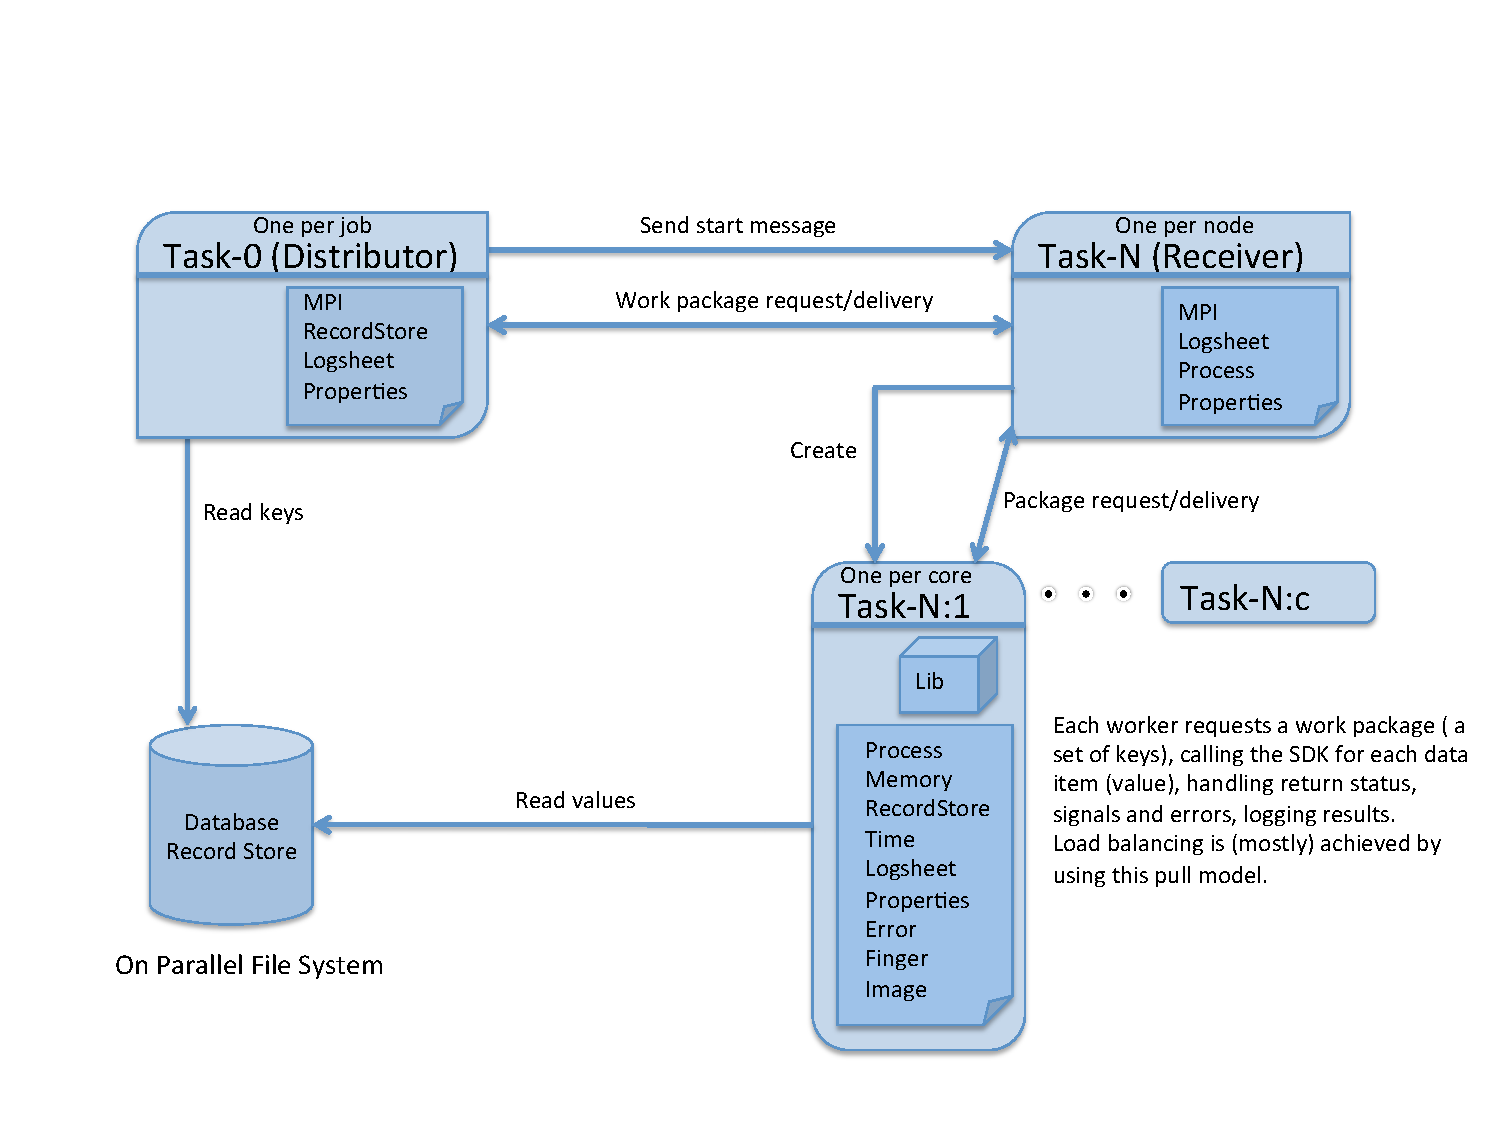
\includegraphics[width=\textwidth]{ParallelJob}
	\caption{MPI Parallel Job Processes and Data Flow}
	\label{fig:paralleljob}
\end{figure}

On the receiving side of the job, the processing is separated into two areas
of responsibility. Each Task-N is responsible for managing the workers
(Task-N:1 \ldots Task-N:c) by starting them, accepting work requests, and
sending a command to have them shut down when the job finishes. Each worker
is responsible for consuming the contents of the work packages; that
implementation is done in the application.

The partitioning of responsibility enables two features of the Framework.
First, a worker process can handle signals or other errors and decide to
shutdown without affecting the rest of the job. This capability is important
when testing ``black-box'' software where function calls cannot be trusted.

Second, each Task-N can perform some work before creating the workers. One
example is the loading of a large data set into memory; again, this is done
within the application. Because Task-N calls the POSIX function \code{fork()}
to create the workers, each worker inherits the work done by Task-N. In the
case of a memory load, each worker now has that memory mapped into it's address
space. See~\secref{sec-workpackageprocessor} for more details.

\section{Work Package}
\label{sec-workpackage}

A \class{WorkPackage} object wraps a simple container of data
with some access methods. There is no information in this class pertaining to
the nature or format of the data; it is simply treated as an array of unsigned
integer values. However, clients of the class can store a value, the ``number
of elements'', that is transmitted along with the package. This value only
has meaning to the client, and is usually equivalent to the number of
larger-sized components making up the package. For example, this value may
be the number of records contained in the package. It is up to the client
of \class{WorkPackage} to understand how to separate the array into components.

The classes \class{RecordStoreDistributor} (\secref{sec-recordstoredistributor})
and \class{RecordProcessor} (\secref{sec-recordprocessor})
are examples of \class{WorkPackage} clients that insert and remove data from
a work package.

\section{Distributor}
\label{sec-workpackagedistributor}

The \class{Distributor} is an abstract class than encapsulates the MPI
functionality and is responsible for distributing work packages to other
elements within the MPI job (the receivers). However, this class
is also responsible for coordinating the startup and shutdown of the receiver
tasks. MPI messages are used for this coordination. An MPI job may fail to
start if the distributor fails to initialize, or if none of the receivers
initialize.

One method of the \class{Distributor} class, \code{createWorkPackage()},
is implemented by child classes. This method creates a single work package
with the knowledge of how the elements of the package are to be stored
in the package's data buffer. \class{RecordStoreDistributor} is an
implementation of \class{Distributor}.

\subsection{Record Store Distributor}
\label{sec-recordstoredistributor}

\class{RecordStoreDistributor} reads records from a \class{RecordStore},
packs record keys, and optionally, values into a \class{WorkPackage}. This
class inherits all of the MPI communication, intra-job coordination, logging,
and other aspects of the \class{Distributor} parent class.

An application can create an instance of a \class{RecordStoreDistributor}
with the name of a record store in order to distribute records for
processing across the MPI job. \lstref{lst:mpiappmain} shows an
example section of code to create a record store distributor. In this
type of application there is no need for the application code to refine
any of the Framework classes.

\section{Receiver}
\label{sec-workpackagereceiver}

The \class{Receiver} class encapsulates all the MPI messaging needed to
participate in the MPI job as the receiver of data to be processed. In
addition, this class is responsible for starting other processes that
perform work on the actual data from the work package.

It is expected, as part of the MPI job, that a single receiver process
will be started on each node in the job. More than one can be started,
however. Each receiver starts one or more child processes to
consume data. The receiver monitors each worker process and
will instruct them to shut down when the job is finished (no more data),
early termination signals are received, or in the case of errors
encountered by the receiver.

By keeping the data consumers as separate processes, the receiving half
of the MPI job can be more robust as a premature termination of a worker
process (due to memory corruption, for example) will not affect other
workers.

\section{Work Package Processor}
\label{sec-workpackageprocessor}

The \class{WorkPackageProcessor} class is pure-virtual and provides the
interface for any class that uses a \class{WorkPackage} to receive data from
the MPI Framework.
\class{WorkPackageProcessor} also maintains a \class{Logsheet} object which
can be used by subclasses to store log messages.

Implementations of this class can be considered to have dual responsibilities.
First is the management of common state used by all workers (Task-N:c in
\figref{fig:paralleljob}); creating state data shared by all workers, for
example.
Second, as a factory to create a package consumer for the worker process.

The \code{performInitialization()} method is called before the \class{Receiver}
object forks and creates the worker processes. The application can use this
function to load a large data set into memory (taking advantage of copy-on-write
memory semantics present in most modern operating systems), or perform any
node-local setup that should only be done once the MPI job has begun.

\code{newProcessor()} returns a new instance of the package processor.
This method is called by the Framework when a new process is started by the
receiver to consume work packages sent by the distributor. This method is a
factory, creating new instances of the \class{WorkPackageProcessor}
implementation. Therefore, it must create a ``fully-formed'' object that may
have different state than that created by the class constructor. An example
would be creating an output log file with record information.
This output file would not be created in the constructor because the
object returned from that will not process a work package; it is the factory
object.

It is the
responsibility of the \code{newProcessor()} method to ensure there is no
resource contention between instances of this class, as the methods of this
object will be executed within a separate process. The
\code{MPI::generateUniqueID()} function can be used to create a name string
that to identify the process.

\subsection{Record Processor}
\label{sec-recordprocessor}
\class{RecordProcessor} is a partial implementation of 
\class{WorkPackageProcessor} and defines the \code{processWorkPackage()}
of the \class{WorkPackageProcessor} interface; other methods are declared as
pure-virtual and must be implemented by a child class. In addition,
\class{RecordProcessor} declares a new pure-virtual method,
\code{processRecord()} to be implemented by a subclass to process a single
record from the record store. In summary, \class{RecordProcessor} removes
records from the work package to be processed within the subclass,
which is defined by the application.
See~\lstref{lst:mpiappclasses} and \lstref{lst:mpiappimpl} for a example of
such an implementation.

\section{MPI Resources}
\label{sec-mpiresources}
Every MPI job depends on a set of properties contained within a text file.
These properties are read into a \class{Properties} object contained within
the \class{Resources} object.

The core MPI classes (\class{Distributor} and \class{Receiver}) use these
properties:
\begin{description}
\item[Workers Per Node] Used by the receiver process to start the
required number of workers;
\item[Logsheet URL] Use by distributor and receiver processes
(and children) to open the log.
\end{description}

The \verb=Logsheet URL= property is optional, and if present all MPI Framework
trace messages will be written to the specified logging target. Two types of
\URL schemes are allowed: \verb=file://= and \verb=syslog://=, corresponding
to the types of \class{Logsheet} classes (\secref{sec-logging}) in the
Framework.

Subclasses and other components of the MPI Framework may add properties as
needed, usually to the same file as the above properties. Record-based jobs
(using \class{RecordStoreDistributor} and \class{RecordProcessor}), for example,
have these additional properties:

\begin{description}
\item[Input Record Store] The input record store;
\item[Chunk Size] How many record keys or key-value pairs to place into a
work package.
\end{description}

For a record store job, an example properties file might be:
\begin{verbatim}
Input Record Store = test.rs
Chunk Size = 7
Workers Per Node = 3
Logsheet URL = file://mpi.log
\end{verbatim}

Applications can add one or more properties to the file as needed. One example
would be a URL for a Logsheet used only by the application.

\section{MPI Runtime}
\label{sec-mpiruntime}

The \class{Runtime} class is the interface between the application and the
MPI runtime environment. The \code{argv} and \code{argc} parameters
to the \code{main()} function as passed through to the \class{Runtime}
object, then onto the core OpenMPI functions. The \class{Runtime} object 
also sets up a signal handler for the job, and starts the \class{Distributor}
and \class{Receiver} processes.  A method is also provided for the application
to abort the MPI job, providing for a somewhat clean shutdown.

On of the key features of an MPI job under the Framework is premature shutdown
with minimal loss of work. Three types of exit condition can be set by sending
a signal to the distributor, receiver or worker processes. 

\begin{description}
\item[SIGQUIT] Exit when the current work package is exhausted;
\item[SIGINT] Exit when the current work item is finished (``quick exit'');
\item[SIGTERM] Exit immediately (``termination exit'').
\end{description}

For the normal exit and quick exit cases, a clean shutdown is performed for
the distributor, receivers, and all worker processes. For term exit, each
worker process is terminated immediately and therefore cannot finish processing
the current work item. However, distributors and receivers will shutdown in a
clean manner.

Any of the signals can be sent to the distributor process, which then sends
messages to the receivers. In addition, if a signal is sent to a receiver or
worker process, only that process (receiver or worker) is affected, but the
termination condition is communicated ``up'' the chain. By selectively sending
signals to certain processes, a user can shutdown the entire job (send to the
distributor), an entire node (send to the receiver on that node), or a single
worker. A worker receiving a signal sends a message back to the receiver.
Likewise, a receiver will communicate the shutdown state back to the
distributor.

In addition to sending signals from outside the process, a worker can shutdown
itself or the entire job through exceptions. Any type of exception thrown
from within a worker will cause that individual worker to shutdown, and its
status will be communicated up the chain. A special type of exception,
\class{TerminateJob}, will shutdown the individual worker, and additionally
communicate up the chain to the distributor that all other workers should
immediately exit. Throwing \class{TerminateJob} from a worker is similar in
result to sending \texttt{SIGTERM} to a distributor.

\section{Logging}
\label{sec-mpilogging}
In order to aid tracing and debugging of a parallel job, the MPI Framework
can be configured to write trace messages to the log storage. These trace
messages are logged as debug messages instead of normal entries.
The type and location of the log is given to the 
Framework by using a URL as a property when starting the MPI
job (see~\secref{sec-mpiresources}).

When the URL for a log is the {\tt file://} type, the MPI Framework will create
several log files on the node where it runs. The reason for this is that during
\class{Receiver} processing, one or more worker processes are created in
addition to the main receiver process. Each of these processes requires
exclusive access to the file-based log sheet in order to avoid conflicts with
the log entry commitment.
The log files will be named with the property value
as a prefix, and the hostname/MPI task number/process ID added as a suffix.
For example, if the property is \verb=file://mpijob.log=, a log file might
have a name of \verb=mpijob.log-node01-1-12345=.

To aid logging within the application, access to the \class{Logsheet} opened
by the Framework is available via the class whose interface is implemented
within the application, \class{WorkPackageProcessor}, for example.

Two wrapper functions, \code{MPI::logMessage()} and \code{MPI::logEntry()},
are provided in order to ``safely'' log. These functions handle all errors
from the \class{Logsheet} object, and will turn off log message commitment
once an error occurs. The Framework and application can continue processing.

\section{MPI Framework Applications}
\label{sec-mpiapp}

An application of the MPI Framework is responsible for implementing several
functions declared in the Framework, requiring subclassing of the MPI classes.
In this section an example application that processes records from a store will
be described. 

\lstref{lst:mpiappclasses} shows the header file that declares a subclass of
\class{RecordProcessor}. The \code{newProcessor()},
\code{performInitialization()}, and \code{processRecord()} methods are those
required to complete an implementation of \class{RecordProcessor}.
A memory buffer pointer is managed with a smart pointer object.

\begin{lstlisting}[caption={MPI Framework Application Classes}, label=lst:mpiappclasses]
class TestRecordProcessor : public BiometricEvaluation::MPI::RecordProcessor {
public:
        /**
         * @brief
         * The property string ``Logsheet URL''.
         */
        static const std::string RECORDLOGSHEETURLPROPERTY;

        static const uint32_t SHAREDMEMORYSIZE = 2048;

        TestRecordProcessor(
            const std::string &propertiesFileName);
        ~TestRecordProcessor();

        std::shared_ptr<BE::MPI::WorkPackageProcessor>
        newProcessor(std::shared_ptr<BE::IO::Logsheet> &logsheet);

        void
        performInitialization(std::shared_ptr<BE::IO::Logsheet> &logsheet);

        void processRecord(const std::string &key);

        void processRecord(
            const std::string &key,
            const BE::Memory::uint8Array &value);

protected:
private:
        std::shared_ptr<BE::IO::Logsheet> _recordLogsheet;
        std::shared_ptr<char> _sharedMemory;
        uint32_t _sharedMemorySize;
};

\end{lstlisting}

Next, \lstref{lst:mpiappimpl} shows the implementation of the class methods. In
this simple example, each record is acknowledged with a log entry.

Also shown in several of the methods is the use of the \class{Logsheet} object
provided to the application by the Framework, along with wrapper functions,
\code{logMessage()} and \code{logEntry()}.

The application also creates its own
\class{Logsheet} object in order to separate Framework log messages from the
application messages when processing the actual record. In error cases, the
Framework log is used in order to keep the set of calls from the Framework
to the application in sequence and package processing together.

A common memory buffer is allocated in \code{performInitialization()} method,
and this buffer's pointer is copied to each processing instance in the
\code{newProcessor()} method. Access to this common memory is shown in each
\code{processRecord()} method. The actual memory buffer is not copied because
the Framework will invoke the system call \code{fork()} which results in all
memory of the parent process being copied into the child. 

\begin{lstlisting}[caption={MPI Framework Application Implementation}, label=lst:mpiappimpl]
#include <be_mpi_receiver.h>
#include <be_mpi_recordstoredistributor.h>
#include <be_mpi_runtime.h>

#include "test_be_mpi.h"

using namespace BiometricEvaluation;

static const std::string DefaultPropertiesFileName("test_be_mpi.props");

/*
 * Implementations of the MPI RecordProcessor class interface.
 * Calls the parent constructor to manage the properties file name.
 */
TestRecordProcessor::TestRecordProcessor(
    const std::string &propertiesFileName) :
    RecordProcessor(propertiesFileName)
{
}

TestRecordProcessor::~TestRecordProcessor()
{
}

/*
 * Factory object: Log our call and set up the shared memory buffer.
 */
void
TestRecordProcessor::performInitialization(
    std::shared_ptr<IO::Logsheet> &logsheet)
{
        this->setLogsheet(logsheet);

        /*
         * Set up the memory that will be shared across all instances.
         */
        char *buf = (char *)malloc(SHAREDMEMORYSIZE);
        strcpy(buf, "SHARED MEMORY");
        this->_sharedMemorySize = SHAREDMEMORYSIZE;
        this->_sharedMemory = std::unique_ptr<char>(buf);

        *logsheet.get() << std::string(__FUNCTION__) << " called: ";
        *logsheet.get()
            << "Shared memory size is " << this->_sharedMemorySize
            << " and contents is [" << buf << "]";
        BE::MPI::logEntry(*logsheet.get());
}

/*
 * Factory object: Create a new instance of the TestRecordProcess
 * that will work on work package records. Each instance gets
 * its own instance of the log sheet.
 */
std::shared_ptr<BiometricEvaluation::MPI::WorkPackageProcessor>
TestRecordProcessor::newProcessor(
    std::shared_ptr<IO::Logsheet> &logsheet)
{
        std::string propertiesFileName =
            this->getResources()->getPropertiesFileName();
        TestRecordProcessor *processor =
            new TestRecordProcessor(propertiesFileName);
        processor->setLogsheet(logsheet);

        /*
         * If we have our own Logsheet property, and we can open
         * that Logsheet, use it for record logging; otherwise,
         * create a Null Logsheet for these events. We use the
         * framework's Logsheet for tracing of processing, not
         * record handling logs.
         */
        std::string url;
        std::unique_ptr<BE::IO::PropertiesFile> props;
        try {   
                /* It is crucial that the Properties file be
                 * opened read-only, else it will be rewritten
                 * when the unique ptr is destroyed, causing
                 * a race condition with other processes that
                 * are reading the file.
                 */
                props.reset(new BE::IO::PropertiesFile(
                    propertiesFileName, IO::READONLY));
                url = props->getProperty(
                    TestRecordProcessor::RECORDLOGSHEETURLPROPERTY);
        } catch (BE::Error::Exception &e) {
                url = "";
        }
        processor->_recordLogsheet = BE::MPI::openLogsheet(
            url, "Test Record Processing");
        processor->_sharedMemory = this->_sharedMemory;
        processor->_sharedMemorySize = this->_sharedMemorySize;

        std::shared_ptr<BiometricEvaluation::MPI::WorkPackageProcessor> sptr;
        sptr.reset(processor);
        return (sptr);
}

/*
 * Helper function to log some information about a record.
 */
static void
dumpRecord(
    BE::IO::Logsheet &log,
    const std::string key,
    const Memory::uint8Array &val)
{
	log << "Key [" << key << "]: ";
	/* Dump some bytes from the record */
        for (uint64_t i = 0; i < 8; i++) {
                log << std::hex << (int)val[i] << " ";
        }
        log << " |";
        for (uint64_t i = 0; i < 8; i++) {
                log << (char)val[i];
        }
        log << "|";
        BE::MPI::logEntry(log);
}

/*
 * The worker object: Log to the Framework Logsheet, obtain the data for
 * the record, and log some information to the record Logsheet.
 */
void
TestRecordProcessor::processRecord(const std::string &key)
{
        BE::IO::Logsheet *log = this->getLogsheet().get();
        
        if (this->getResources()->haveRecordStore() == false) {
                BE::MPI::logMessage(*log, "processRecord(" + key + ")"
                    + " called but have no record store; returning.");
                return;
        }
        *log << "processRecord(" << key << ") called: ";
        char *buf = this->_sharedMemory.get();
        *log << "Shared memory size is " << this->_sharedMemorySize
            << " and contents is [" << buf << "]";
        BE::MPI::logEntry(*log);

        Memory::uint8Array value(0);
        std::shared_ptr<IO::RecordStore> inputRS =
            this->getResources()->getRecordStore();
        try {
                inputRS->read(key, value);
        } catch (Error::Exception &e) {
                *log << string(__FUNCTION__) <<
                    " could not read record: " <<
                    e.whatString();
                return; 
        }
        /*
         * Log record info to our own Logsheet instead of
         * the one provided by the framework.
         */     
        BE::IO::Logsheet *rlog = this->_recordLogsheet.get();
        dumpRecord(*rlog, key, value);
}

/*
 * The worker object: Log to the Framework Logsheet, and log some record
 * information to the record Logsheet.
 */
void
TestRecordProcessor::processRecord(
    const std::string &key,
    const BiometricEvaluation::Memory::uint8Array &value)
{
        BE::IO::Logsheet *log = this->getLogsheet().get();
        *log << "processRecord(" << key << ", [value]) called: ";
        char *buf = this->_sharedMemory.get();
        *log << "Shared memory size is " << this->_sharedMemorySize
            << " and contents is [" << buf << "]";
        BE::MPI::logEntry(*log);

        /*
         * Log record info to our own Logsheet instead of
         * the one provided by the framework.
         */
        BE::IO::Logsheet *rlog = this->_recordLogsheet.get();
        dumpRecord(*rlog, key, value);
}

\end{lstlisting}

\begin{lstlisting}[caption={MPI Framework Application Main}, label=lst:mpiappmain]
int
main(int argc, char* argv[])
{
        /*
         * It is important that the MPI runtime environment be started
         * prior to any other activity that may result in premature
         * termination. Therefore, participate in the MPI environment, but
         * don't create a Receiver or Distributor until any local items
         * are take care of.
         */
        MPI::Runtime runtime(argc, argv);

        std::unique_ptr<MPI::RecordStoreDistributor> distributor;
        std::unique_ptr<MPI::Receiver> receiver;
        std::shared_ptr<TestRecordProcessor> processor;

        /*
         * If there is any argument to the program, use keys only as the
         * record distribution method. Otherwise, use keys and values.
         */
        bool includeValues;
        if (argc == 1) {
                MPI::printStatus("Test Distributor and Receiver, keys only");
                includeValues = false;
        } else {
                MPI::printStatus("Test Distributor and Receiver, keys and values");
                includeValues = true;
        }
        try {
                distributor.reset(
                    new MPI::RecordStoreDistributor(propFile, includeValues));

                processor.reset(new TestRecordProcessor(propFile));

                receiver.reset(new MPI::Receiver(propFile, processor));

                runtime.start(*distributor, *receiver);
                runtime.shutdown();
        } catch (Error::Exception &e) {
                MPI::printStatus("Caught: " + e.whatString());
                runtime.abort(EXIT_FAILURE);
        } catch (...) {
                MPI::printStatus("Caught some other exception");
                runtime.abort(EXIT_FAILURE);
        }

        return (EXIT_SUCCESS);
}

\end{lstlisting}
